\section{Experimentation and results}\label{experimentation}
In this section, we present the performance of our prediction
 model for Malaria occurrecne through an analysis of the results
 of the experimentations we have conducted on real-world datasets
and a semi-synthetic dataset. We start by presenting our experimentation setting.
 
% Experimentation setting
\subsection{Experimentation setting}
We ran tests on three different datasets using the Python Implementation of the logistic regression function.
To impute missing data, we have used the R package of the algorithm missForest.

% Our datasets
\subsubsection{Our datasets.}
We collected and used a real-world patient dataset from the different health points which were set during the Grand Magal of Touba in 2016.
We also generated and used two variants of this real-world dataset. The description of the characteristics of our raw real-world dataset, as well as the  data preparation
pipeline that we have proposed in order to clean, normalize and impute information, are given in Section \ref{data_prep}; we refer to this cleaned and complete real-world
patient dataset by \textsc{DT1}. 

We generated the first variant, denoted by \textsc{DT2}, of the raw real-world patient dataset by 
removing records with missing attributes, instead of using an imputation algorithm that will predicts 
values for missing information. Such a variant will help to study the impact of removing records with 
missing values in the prediction accuracy.
 
The second variant, called \textsc{DT3}, is a semi-synthetic dataset which has been set up by using a 
sampling strategy over our raw real-world dataset. Indeed when we have performed some explanatory analysis 
on the real-world dataset have been revealed that the dataset was not balanced, i.e. it shows strong between
class imbalance; the amount of records about patients suffering from Malaria was largely less than the number
of patients that do not suffer from Malaria as shown in Figure \ref{records_class}. Harnessing sampling approaches may enbale to obtain a balanced 
semi-dataset regarding the two classes to predict. To solve our problem of imbalanced dataset, we used the 
algorithm SMOTE \cite{Wa06}, which is a synthetic minority oversampling technique, through its Python implementation
in the  package \emph{imbalanced-learn} \cite{Gu17}. SMOTE consists of predicting a sample of synthetic dataset based on 
the value of the minority class of the targeted class (here the attribute Diagnostic). It randomly chooses the k-nearest 
neighbours of a given record in order to randomly create new observations.
 We have applied an over-sampling of the minority class into our patient 
dataset for generating  a semi-synthetic dataset \textsc{DT3} containing the same number of records for both classes.  

% distribution of records by class
\begin{figure}[h]
\centering
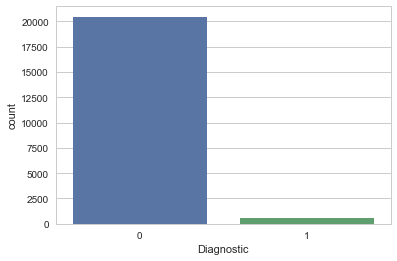
\includegraphics[width=0.6\textwidth]{images/imbalanced_dataset}
\label{records_class}\caption{The number of records by class}
\end{figure} 

% Implementation of the logistic model
\subsubsection{Prediction model setting.}
In order to set up our logistic regression-based classification model, we rely on the Python implementation of the logistic regression in the \emph{sklearn} library\footnote{https://scikit-learn.org/stable/modules/generated/sklearn.linear\_model.LogisticRegression.html}.
This python package defines the logistic regression with the required input parameters, as well as optimization strategies, to properly perform binary 
classification using the best final model. For the purposes of our tests, we have used the following input parameters of the logistic regression:

% input parameters
\begin{itemize}
\item \textbf{random\_state}: it models the seed of the pseudo random number generator to use when shuffling the data. Its value
is set to $0$ as we do not need to shuffle data in our experimentations.
\item \textbf{class\_weight}: weights associated with classes. We set it to \emph{None}, i.e. all classes are supposed to have weight one.
\item \textbf{dual}: dual or primal formulation. Dual formulation is only implemented for l2 penalty with liblinear solver.
This parameter is set to \emph{False} as the number of samples is greater than the number of features.
\item \textbf{fit\_intercept}: useful if a constant (a.k.a. bias or intercept) should be added to the decision function. Consequently,
we fixed the fit\_intercept to \emph{True}.
\item \textbf{intercept\_scaling}: this parameter, set to $1$, is useful only when the solver \textquote{liblinear} is used and fit\_intercept is set to True.
\item \textbf{max\_iter}: maximum number of iterations taken for the solvers to converge.
\item \textbf{multi\_class}: if the option chosen is \textquote{ovr}, then a binary problem is fit.
\item \textbf{n\_jobs}: number of cpu cores used when parallelizing over classes if multi\_class=\textquote{ovr}. This parameter is ignored when the
solver is  set to \textquote{liblinear} regardless whether \textquote{multiclass} is specified or not.
\item \textbf{penalty}: this parameter is used to specify the norm in the pernalization. We fixed the penality to its default value $l2$.
\item \textbf{solver}: it enables to specify the strategy used to solve the optimization underlying our model. For the solver we fix it 
to \emph{liblinear}.
\item \textbf{tol:} tolerance for stopping criteria which is set to $0.0001$.
\item \textbf{verbose}: for the liblinear solver set verbose to any positive number for verbosity.
\item \textbf{warm\_start}: when set to \emph{True}, reuse the solution of the previous call to fit as initialization, otherwise, just erase the
 previous solution. Useless for liblinear solver.
\end{itemize}

As the logistic regression performs a supervised learning we have used 60\% for the training set and 30\% for the test set.

% Performance measures
\subsection{Performance measures}
To evaluate the performance of our prediction approach over the different used datasets, we have computed the precision,
recall (or sensitivity), F-measure, and specificity of the predicted classes. We have also drawn the graph of the Receiver operating 
characteristic of the logistic regression to study its shape.  
The sensitivity, specificity and ROC plot are often used in the medecine domain as performance measures for prediction tasks.

\subsubsection{Precision.}
\subsubsection{Recall.}
\subsubsection{F-measure.} The F-measure, denoted by F$_1$ is a metric that measures the accuracy of a test in statistical analysis of a binary classification.
It is computed using both the precision $p$ and the recall $r$ of the test as the ratio of the number of correct positive results and the
number of all positive results returned by the classifier. 

% F-measure formula
\begin{equation}
F_1 = 2 \times \frac{p\times r}{p + r}
\label{f-measure}
\end{equation}
 
\subsubsection{Specificity.}
\subsubsection{Receiver operating characteristic.} A receiver operating characteristic, or ROC in short, is a graph
 that shows the diagnostic ability of a binary classifier system as its discrimination threshold is varied.
The ROC curve is created by plotting the \emph{true positive rate} (i.e. sensitivity or recall in machine learning) 
against the false positive rate (1 - specifity) at various threshold settings. 

% Analysis of the results
\subsection{Experiments and analysis of the results}


\subsubsection{Experiments with DT1}
\subsubsection{Experiments with DT2}


% results for precision, recall, f1-score
\begin{table}[h]
\centering
\begin{tabular}{cccc}
Precision & Recall & F-measure & \\
\end{tabular}
\end{table}

% the roc curve
\begin{figure}
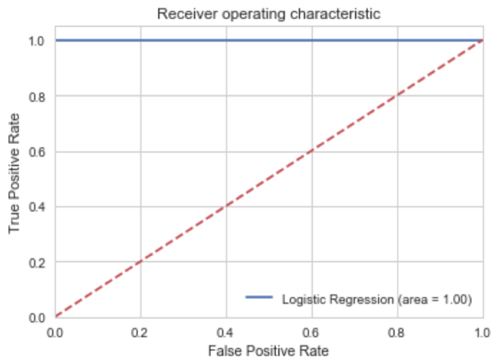
\includegraphics[width=.8\textwidth]{images/curve_roc_dt2}
\end{figure}
\subsubsection{Experiments with DT3}
\subsubsection{Comparative analysis of the results}
